\documentclass[letterpaper, 10 pt]{report}
\usepackage{hyperref}
% For handling graphics
\usepackage{graphicx}
% For multirows in tables
\usepackage{multirow}
% For colors
\usepackage{color}
% For hyperlink
\usepackage{hyperref}
\hypersetup{
    colorlinks,
    linktoc=all,
    citecolor=black,
    filecolor=black,
    linkcolor=black,
    urlcolor=blue
}
\usepackage[margin=1.0in]{geometry}
\usepackage{listings}

\setcounter{secnumdepth}{-2}
% -------------------------------------------------------------------------------------
% TITLE PAGE
% -------------------------------------------------------------------------------------
\begin{document}
\begin{titlepage}
\center
% Headings
\textsc{\LARGE Georgia Institute of Technology}\\[1.5cm]
\textsc{\large Institute for Robotics \& Intelligent Machines}\\[0.5cm]
\textsc{\large Humanoid Robotics Lab}\\[0.5cm]
% Title
\rule{\linewidth}{0.5mm}\\[0.4cm]
{\huge \bfseries DRC-HUBO Operation Manual}\\[0.4cm]
\rule{\linewidth}{0.5mm}\\[1.5cm]
% Author
\textsc{\normalsize M.X. Grey}\\
\textsc{\normalsize Eric Huang}\\
\textsc{\normalsize Andrew Price}\\
\textsc{\normalsize Peter Vieira}\\
\textsc{\normalsize Sungmoon Joo}\\[0.5cm]
\textsc{\normalsize Update 2014.03.12}\\[0.5cm]
% Image
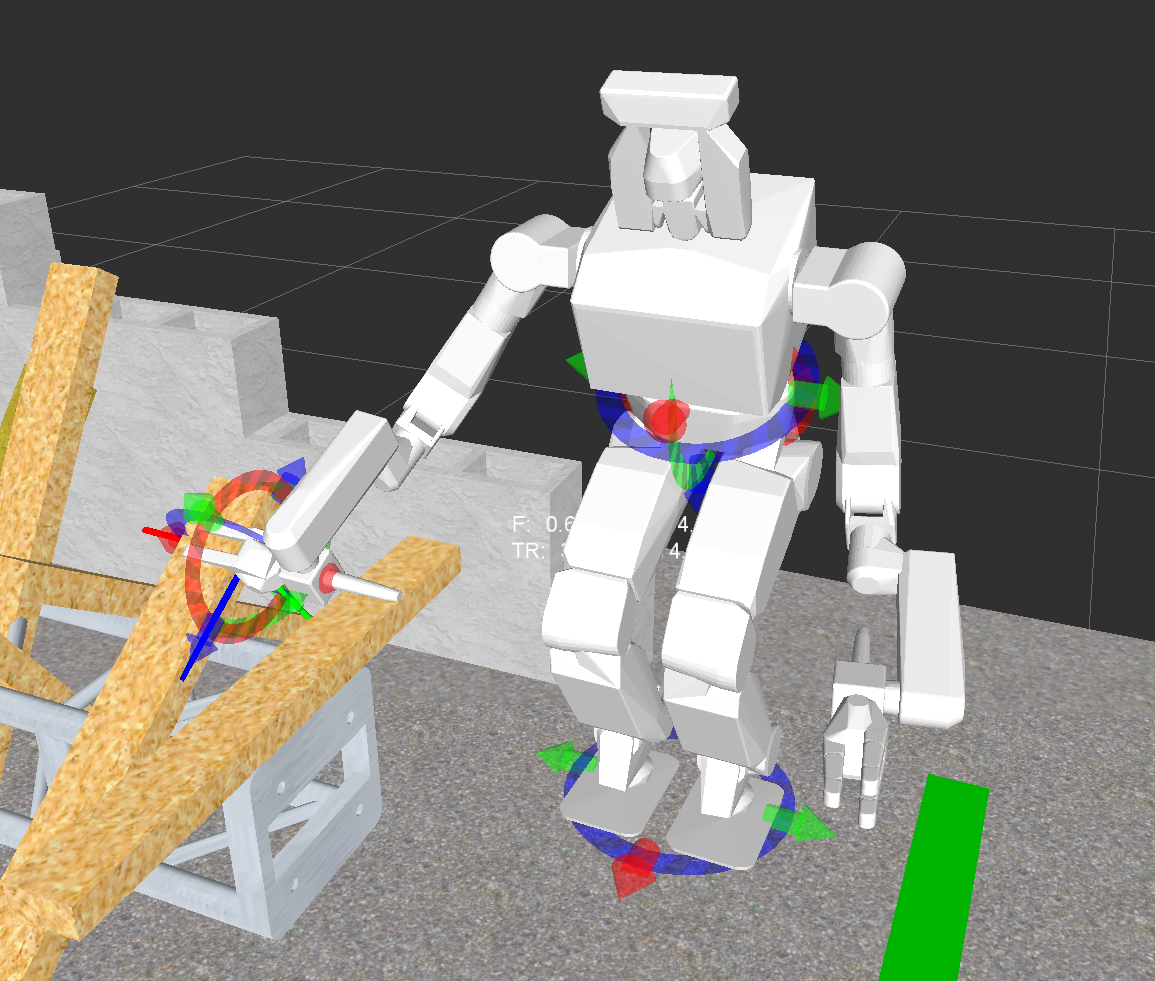
\includegraphics[width=10.0cm]{figures/hubo_keypose_1.png}
% Fill rest of page with whitespace
\vfill
\end{titlepage}


% TABLE OF CONTENTS
% -------------------------------------------------------------------------------------
\tableofcontents
\newpage


% -------------------------------------------------------------------------------------
% CODE REPOS
%
\chapter{Code Repositories}\label{chap:code-repos}
The following code repositories are required in order to execute our tasks using our code. They consist of real-time processes that run on the robot, and code that uses ROS and runs mostly on a local computer.
\section{Main Code}
Code repositories that run in real-time on the robot.
\begin{itemize}
\item hubo\_gt
  \begin{itemize}
	\item \url{https://github.com/golems/hubo_gt}
  \end{itemize}
\end{itemize}
\section{Major Dependencies(To Do: check forked repos)}
\begin{itemize}
  \item \url{https://github.com/golems/hubo-ach} (master, installation required)
  \item \url{https://github.com/arebgun/dynamixel_motor} (master)
  \item \url{https://github.com/hubo/hubo_planning_common} (master)
  \item \url{https://github.com/hubo/hubo_vision_common} (master)
  \item \url{https://github.com/hubo/hubo_ros_core} (master)
  \item \url{https://github.com/hubo/hubo_ros_control} (master)
  \item \url{https://github.com/hubo/hubo_head_description}
   (master)
  \item \url{https://github.com/golems/teleop_toolkit} (master)
\end{itemize}
\section{Minor Dependencies}
Dependencies that can be install with \textit{apt-get install}
\begin{itemize}
  \item ach-utils
  \item autoconf, automake, autoconf-archive, libtool
  \item expat
  \item freeglut3-dev
  \item libboost1.46-dev
  \item libeigen3-dev
  \item libreadline6-dev
  \item ros-groovy-desktop-full (note. catkin workspace \& env. set-up required)
  \item ros-groovy-control-msgs
  \item ros-groovy-libccd
  \item ros-groovy-moveit-msgs
  \item ros-groovy-spacenav-node
  \item ros-groovy-urdf
  \item ros-groovy-urdfdom
  \item libopenni2-dev
\end{itemize}
\section{Vision}
\begin{itemize}
  \item \url{https://github.com/ros-drivers/openni2\_camera} (groovy-devel)
  \item \url{https://github.com/ros-drivers/openni2\_launch} (groovy-devel)
\end{itemize}
\newpage

% -------------------------------------------------------------------------------------
% INSTRUCTIONS
%

\chapter{System Setup}\label{chap:system-setup}
This section describes how to get everything on the operators computer up and running with RViz.
\section{RViz Setup}
\begin{enumerate}
  \item After successfully running \textit{catkin\_make} launch \textit{roscore} by typing the following command into the terminal.
  \begin{lstlisting}
  roscore
  \end{lstlisting}
  \item Then in a second terminal start your RViz session with
  \begin{lstlisting}
  rosrun rviz rviz
  \end{lstlisting}
\end{enumerate}

\pagebreak
\chapter{Operation Instructions}\label{chap:operating-instructions}
This section details how to operate DRC-HUBO from the initialization phase to execution of the tasks. The different phases include \textit{Starting-up HUBO}, \textit{Starting-up Perception}, \textit{Walking}, and \textit{Teleop Manipulation}.
\section{Starting-up HUBO}
This section describes how to start-up HUBO.
\begin{enumerate}
  \item Make sure your computer is connected to the local Humanoids router via Ethernet or to the \textbf{humanoids} or \textbf{humanoids-5} wireless network.
  \item Turn on motor controllers with remote
  \item Connect to HUBO's computer using ssh.
  \begin{lstlisting}[language=bash]
  $ ssh hubo@hubo-ach-beta-1
  	(Note: password: hubo1234)
  \end{lstlisting}
  \item \textbf{IMPORTANT: }Turn on power to the motor control boards before starting the daemons
  \item Now start the daemons from the ssh session connected to HUBO's computer
  \begin{lstlisting}
  $ ssh sudo service hubo-motion teleop
  \end{lstlisting}
  \item On your local computer (outside of the ssh sesion), start a ROS master, launch RViz, start the state publisher and the fullbody\_teleop nodes.
  \begin{lstlisting}[language=bash]
  $ roscore (Terminal 1)
  $ rosrun rviz rviz (Terminal 2)
  $ roslaunch hubo_motion_ros hubo_state.launch (Terminal 3)
  $ roslaunch hubo_motion_ros fullbody_teleop.launch (Terminal 4)
  \end{lstlisting}
  \item Click on the \textit{HuboInitPanel} panel tab.
  \begin{figure}[ht]
    \centering
    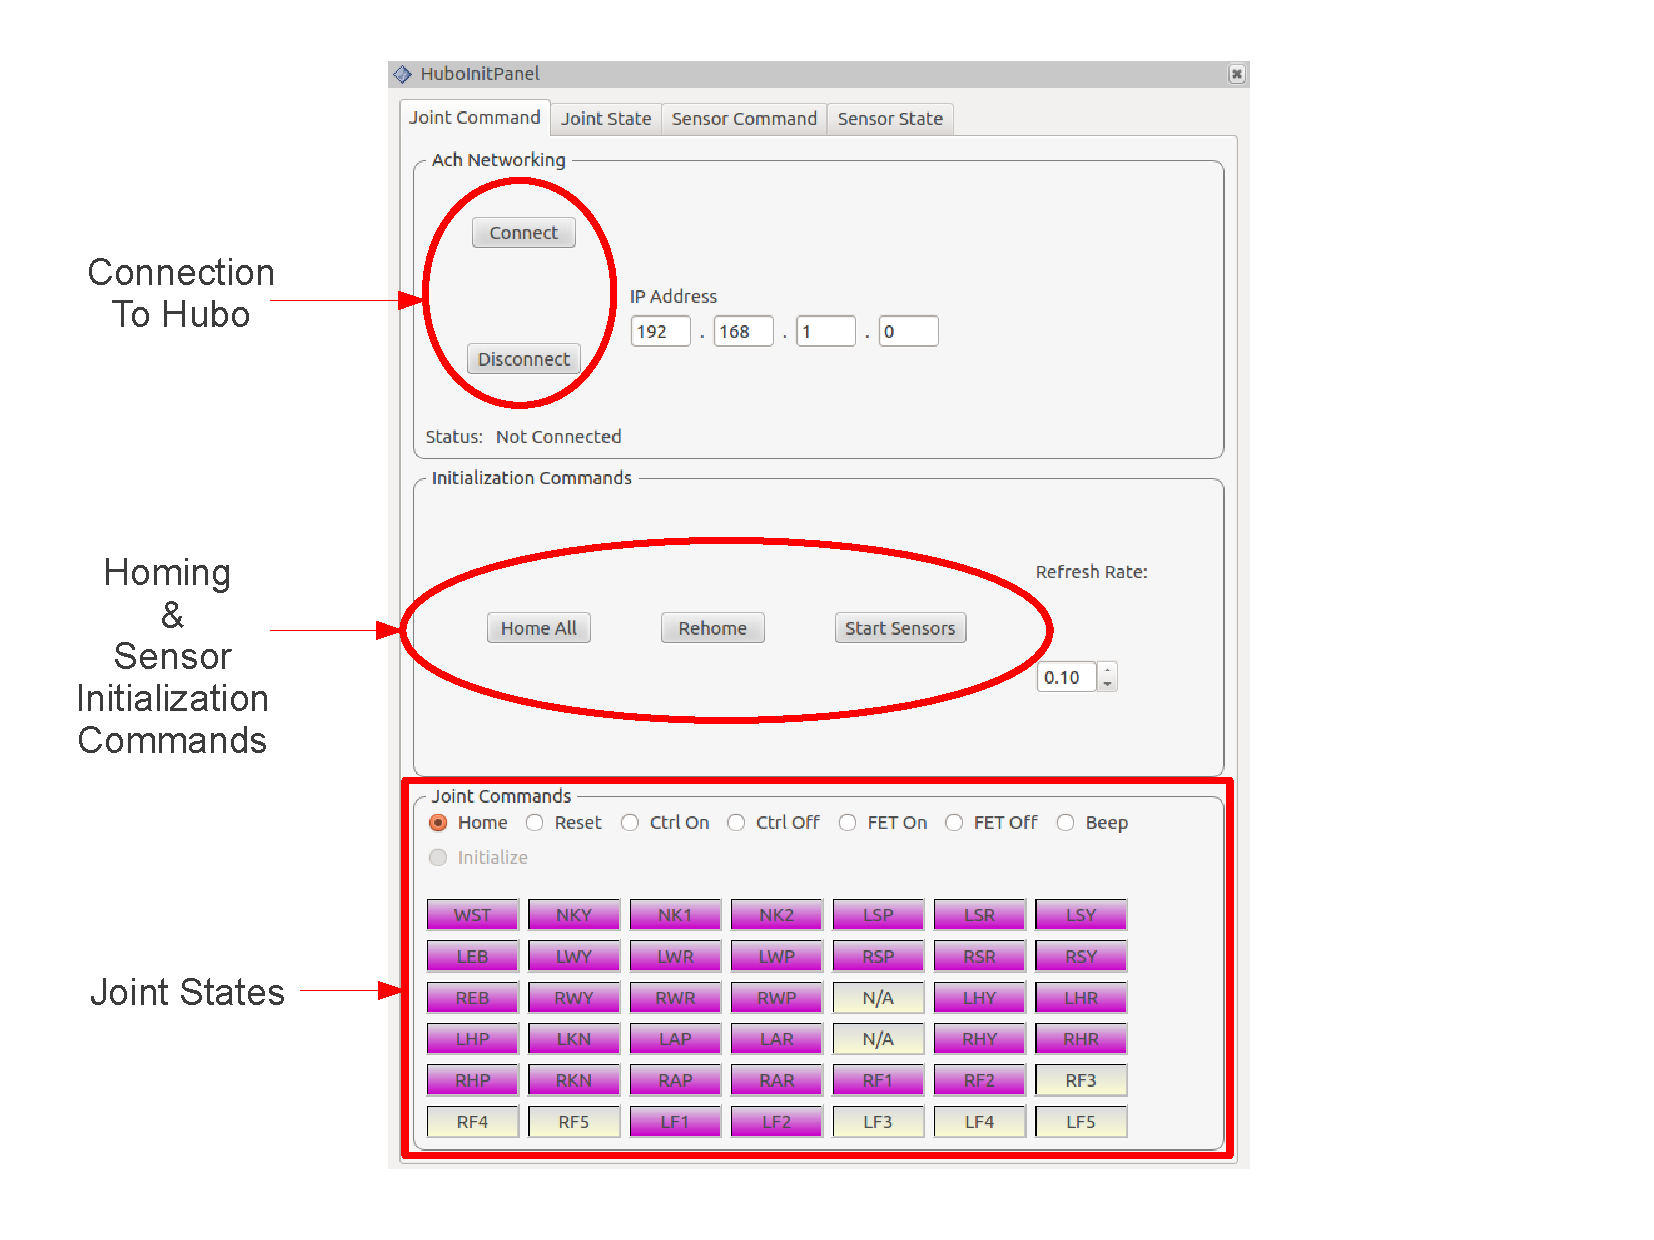
\includegraphics[width=15.0cm]{figures/hubo-init.pdf}
    \caption{Picture of HUBO\_init panel.}
    \label{fig:hubo-init-image}
  \end{figure}
  \item On the \textbf{Joint Command} tab ensure "IP Address" is correct.
  \item Click "Connect" to send and receive ach channels between HUBO's computer and the remote computer. If it won't connect see the Troubleshooting section.
  \item To check if it is indeed connected and receiver ach frames, click on the \textbf{Sensor State} tab in HuboInitPanel and make sure the sensor values are changing. If they are not, then something was most likely done out of order.
  \item Make sure HUBO is sufficiently raised above the ground and click "Home All" to home all of HUBO's joints.
  \item If any active joints do not home, indicated by the color in the \textit{Joint State} section not being gray, click the "Rehome" button. Button color meanings are
    \begin{itemize}
      \item GRAY: homed
      \item PURPLE: not homed
      \item RED: error
      \item WHITE: inactive
    \end{itemize}
  \item If any joints won't home, you can do one of two options:
    \begin{enumerate}
      \item Click the \textit{Reset} radio button and then click the joint(s) that won't home. Then click the \textit{Home} radio button and click the joint(s) that didn't home. Then press the ``Rehome'' button again.
      \item Run ``sudo service hubo-motion stop'', turn off the motor power, wait a moment, turn it back on, and run ``sudo service hubo-motion teleop''. Then try homing again from the beginning. If this doesn't work, HUBO's computer needs to be rebooted and you need to start over from step 1. Basically the CAN line gets corrupted if the daemons are started while the power to the motor control boards is off.
    \end{enumerate}
  \item Once the joints are all homed, press the "Start Sensors" button to initialize the IMU and Force/Torque sensors.
  \item Click on the \textit{Sensor State} tab and ensure the sensor values are updating and are reasonable. If they aren't, then restart the whole process.
  \item Now you click on the \textbf{HuboMotionPanel} tab and click the \textbf{Connect} button.
  \item Click the \textbf{Teleop} button on the top right.
\end{enumerate}

\section{Starting-up Perception} \label{sec:starting-up-perception}
This section is heavily under construction. Generally, what you will need to do is something like this:
  \begin{lstlisting}[language=bash]
    $ roslaunch hubo_drc_vision hubo_openni.launch
  \end{lstlisting}
  
\pagebreak
\section{Camera Calibration} \label{sec:calibration}
In many circumstances, you may find that an approximate camera calibration is insufficient for real manipulation tasks.
In order to alleviate this problem, the intrinsic and extrinsic properties of the camera need to be computed.
For intrinsic calibration, we used the ROS package camera\_calibration (\url{http://wiki.ros.org/camera_calibration}). If using a PrimeSense camera, both the infrared and rgb cameras will need to have their intrinsics calibrated as documented in the package.

For extrinsic calibration, we have written a small subroutine to assist with the calculation.
There are several steps:
\begin{enumerate}
  \item Attach checkerboards to the flat places on the hands. Example checkerboards are provided in the hubo\_gt\_ros/hubo\_drc\_vision/resources folder.
  \item Measure the transform from the hand origin to the checkerboard origin. These values are currently hard-coded for a single checkerboard in the main function of camera\_calib.cpp; this needs to be expanded to accept ROS parameters.
  \item Launch the calibration procedure as follows:
  \begin{lstlisting}[language=bash]
    $ roslaunch hubo_drc_vision calibrate_camera.launch
  \end{lstlisting}
  This will load a list of joint angles from a csv file and play that "trajectory" through the motion pipeline. A second node will monitor the vision system and will compute the least-squares transform that best solves the system of observed and expected points. This transform will be published into TF, and the results can be viewed in RVIZ (use calibration.rviz to automatically configure RVIZ to display the relevant topics).
\end{enumerate}

\pagebreak
\section{Walking}
This section describes how to make HUubo walk. And assumes the robot is already up and running and standing on the ground on two feet.
  \begin{enumerate}
    \item Click on the \textit{HuboWalkPanel} tab.
    \begin{figure}[ht]
      \centering
      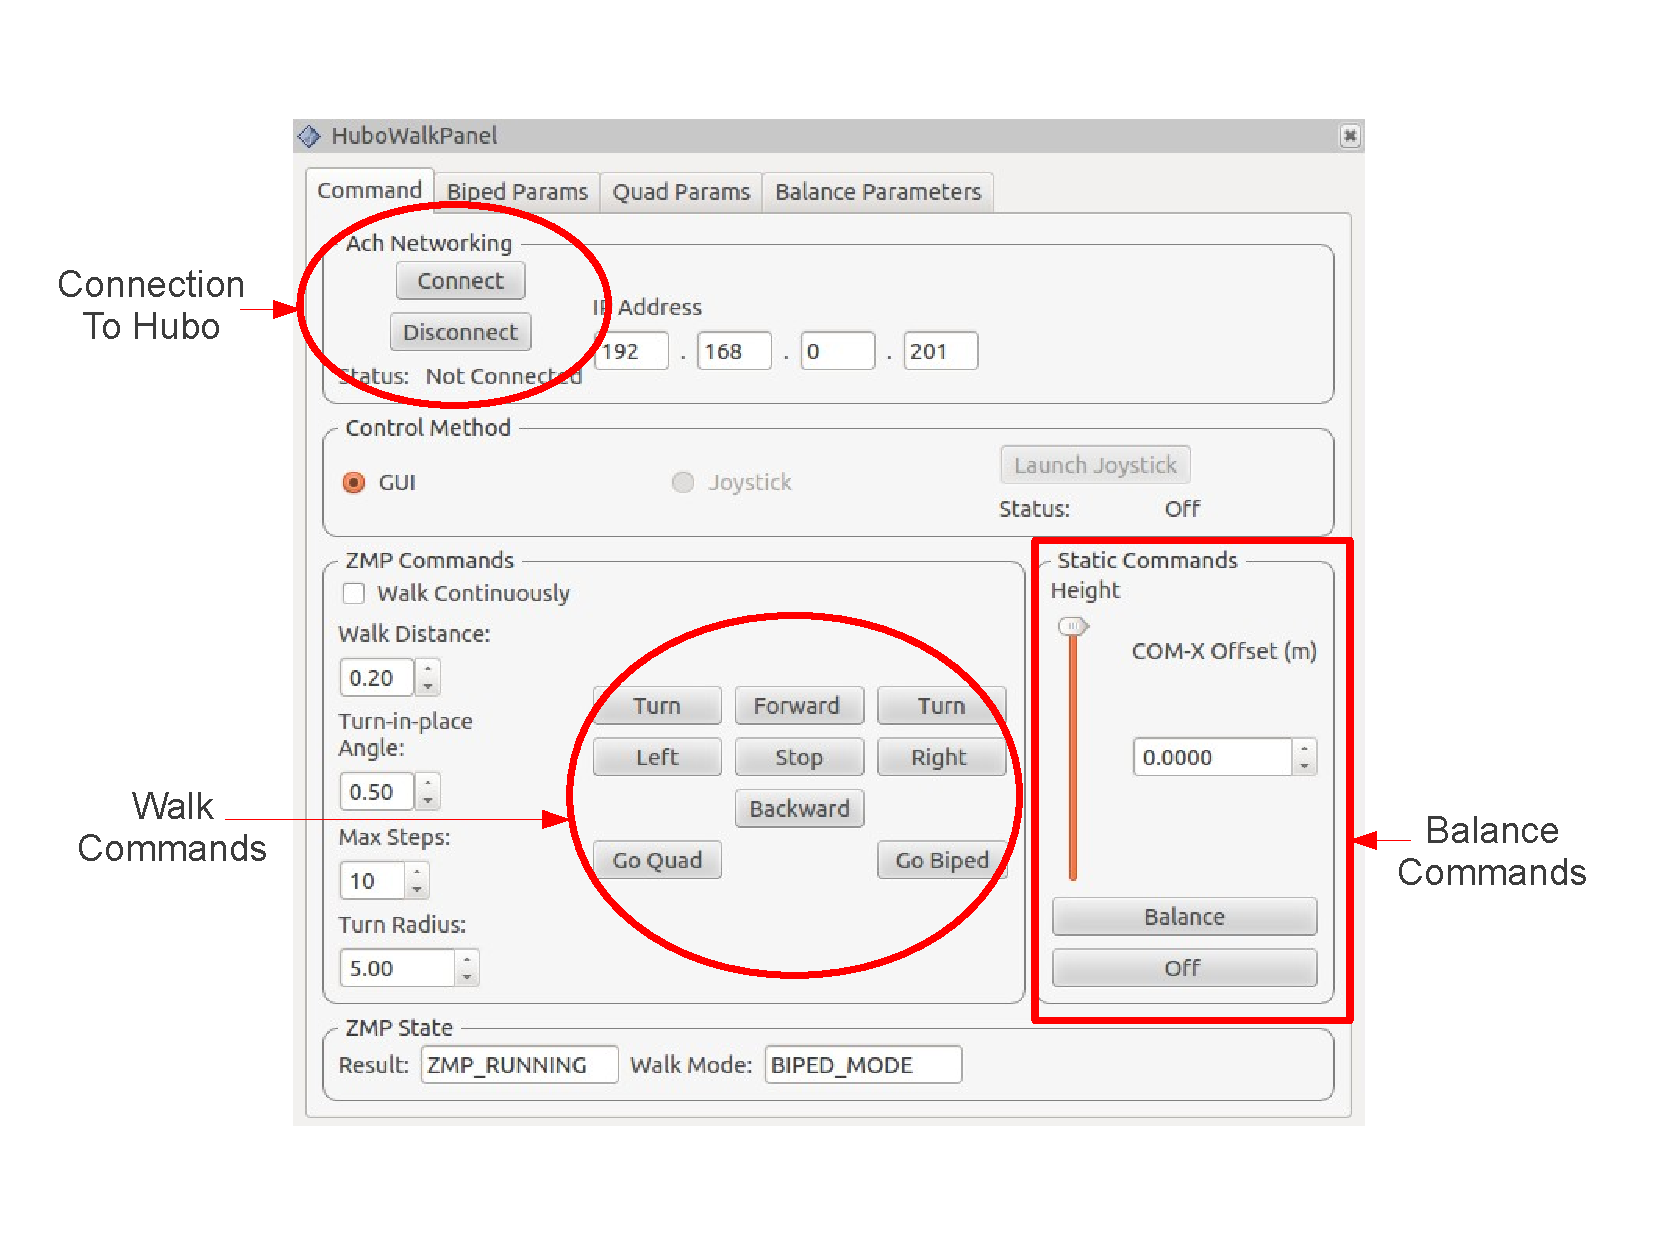
\includegraphics[width=15.0cm]{figures/hubo-walk.pdf}
      \caption{Picture of hubo\_walk panel.}
      \label{fig:hubo-walk-image}
    \end{figure}
    \item Ensure the IP Address is correct.
    \item Click ``Connect'' to send and receive ach channels between HUBO's computer and the remote computer. If it won't connect see the Troubleshooting section.
    \item Based on vision feedback enter desired walk distance, max number of steps, and turn-in-place angle (for turning in place).
    \item Click the ``Go Quad'' button to transition into quadruped mode.
    \item Click the walk command desired to get to your desired goal. (Eventually the interface will use a desired location and orientation, and the ZMP walk generator will create a footstep plan to get there.) The \textit{Walk Continuously} checkbox determines whether or not to walk the specified distance or walk until receiving a stop command. The \textit{ZMP State} section at the bottom of the panel display the state of the ZMP walker generator.
    \item Click ``Go Biped'' to get back up on two feet in order to manipulate objects.
    \item In the \textit{Balance Commands} section of the panel, click "Balance" to go into static balancing mode.
    \item The x-location of the center of mass can be adjusted in the \textit{COM-X Offset (m)} field. Then click the "Balance" button to send the command.
    \item The squat height of the robot can be adjusted by sliding the \textit{Height} slider up and down, which automatically sends the command to the robot.
  \end{enumerate}
  
\pagebreak
\section{Manipulation}
This section describes how to teleoperate HUBO in order to manipulate objects in the environment with either or both arms.
NB: First install all software outlined in \nameref{chap:code-repos}
\begin{enumerate}
  \item If you haven't already, start up ROS
  \begin{lstlisting}[language=bash]
  $ roscore
  $ rosrun rviz rviz
  \end{lstlisting}
  Configuring RViz interface
  \begin{itemize}
    \item If the Displays panel is not visible already, click on the Panels menu and click on Displays.
    \item Under Global Options, set Fixed Frame to /Body\_RAP.
    \item Click Add and scroll to RobotModel. Set topic to robot\_description. Set alpha to 0.5. If the model does not appear, uncheck and check the RobotModel checkbox.
    \item Click Add and scroll to RobotModel. Set topic to robot\_planning\_description. If the model does not appear, uncheck and check the RobotModel checkbox.
    \item Click Add and scroll to Pose. Set Topic to /rh\_pose. Set Axes Length to 0.1 and Axes Radius to 0.01.
    \item Click Add and scroll to TF. Set Marker Scale to 0.1.
    \item Click Add and scroll to InteractiveMarkers. Set Topic to /joint\_controls/update.
  \end{itemize}
  \item Start the teleoperation interface and state feedback
  \begin{lstlisting}[language=bash]
  $ roslaunch hubo_motion_ros fullbody_teleop.launch
  $ roslaunch hubo_motion_ros hubo_state.launch
  \end{lstlisting}
  \item (Optional) Start up Vision system as discussed in \nameref{sec:starting-up-perception}.
\end{enumerate}
  \begin{figure}[ht]
    \centering
    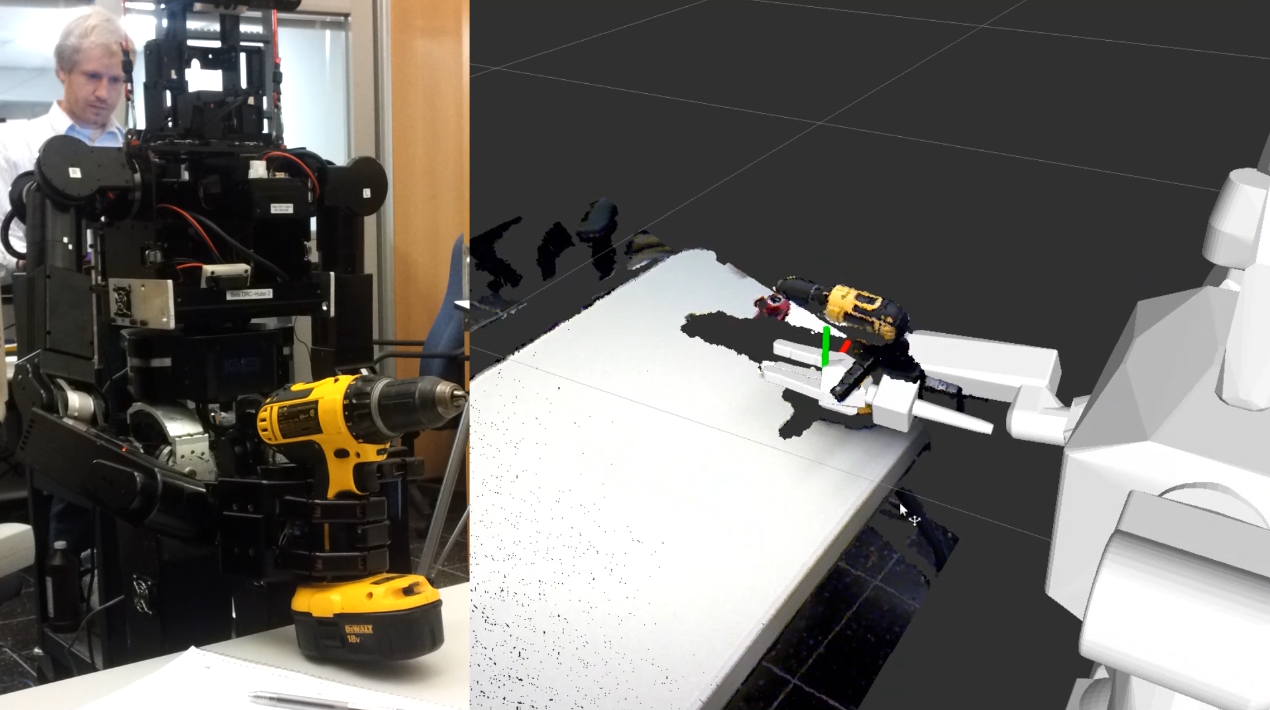
\includegraphics[width=12.0cm]{figures/pickup-drill-rviz}
    \caption{Picture of teleoperation of picking up a drill.}
    \label{fig:pickup-drill-rviz-image}
  \end{figure}
  \begin{figure}[ht]
    \centering
    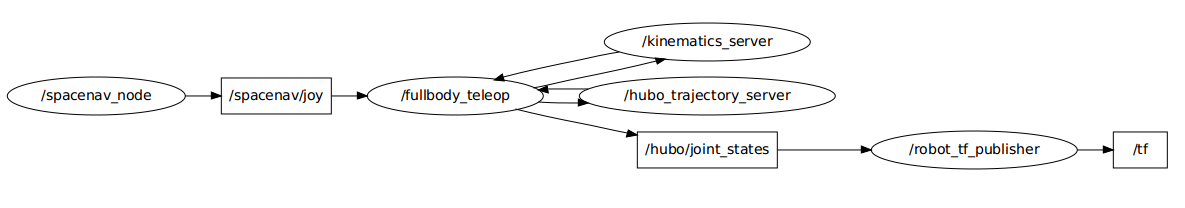
\includegraphics[width=12.0cm]{figures/teleop-rosgraph}
    \caption{Simplified ROS Graph created by fullbody\_teleop.launch.}
    \label{fig:teleop-rosgraph-image}
  \end{figure}

% -------------------------------------------------------------------------------------
% Upocoming Features
%
\pagebreak
\section{Upcoming Features}
This section lists the features which we intend to implement and stabilize prior to the DRC. Many of these
features we consider to be crucial for successful teleoperation of the task.

\begin{enumerate}
  \item End effector Force-Torque workspace control
  \item Cooperative dual-arm manipulation
  \item Simultaneous dual-arm manipulation
  \item Human-assisted planning phase for collision avoidance
\end{enumerate}


% -------------------------------------------------------------------------------------
% TROUBLESHOOTING
%
\clearpage
\chapter{Troubleshooting}\label{chap:troubleshooting}
\begin{table}[ht]
  \centering
  \caption{Troubleshooting Table}
  \begin{tabular}{|p{4.5cm}|p{4.5cm}|p{4.5cm}|} \hline
    \multicolumn{1}{|c|}{Symptom} & \multicolumn{1}{|c|}{Causes} & \multicolumn{1}{|c|}{Solution} \\ \hline
    Can't ssh to HUBO \end{enumerate} & \begin{enumerate} \item Connect to the correct network. \item Ensure daemons are running by typing \textit{ps aux $|$ grep daemon} or restarting HUBO and running \textit{sudo service hubo-motion start}. \end{enumerate} \\
    \hline
    Receiving ACH\_OVERFLOW from rviz command. \newline HuboInitPanel joint names don't showing up correctly. & Don't have matching or most up-to-date installs of hubo-ach, hubo-motion-rt, hubomz or possible another repo. & Make sure you are on the right branch in each repo and reinstall on both machines. \\
    \hline
    Robot homes only the upper or lower body, or neither. & CAN line got corrupted. & Shutdown and turn off the HUBO PC and turn it back on and try again. \\
    \hline
  \end{tabular} \label{tbl:troubleshooting}
\end{table}


% -------------------------------------------------------------------------------------
% REFERENCES
% -------------------------------------------------------------------------------------
%\bibliography{}

% -------------------------------------------------------------------------------------
% END DOCUMENT
% -------------------------------------------------------------------------------------
\end{document}
